\documentclass[10pt]{article}
\usepackage[margin=0.65in]{geometry}
\usepackage[T1]{fontenc}
\usepackage{lmodern}
\usepackage{microtype}
\usepackage{amsmath,amssymb}
\usepackage{booktabs,array,tabularx}
\usepackage{listings}
\usepackage{xcolor}
\usepackage[hidelinks]{hyperref}
\usepackage{enumitem}
\usepackage{titlesec}
\usepackage{tikz}
\usetikzlibrary{arrows.meta,positioning,calc}

\setlist{nosep,leftmargin=1.4em}
\titlespacing*{\section}{0pt}{1.1ex}{0.5ex}
\titlespacing*{\subsection}{0pt}{0.9ex}{0.3ex}
\setlength{\parskip}{0.35em}
\setlength{\parindent}{0pt}

\lstdefinestyle{code}{
  basicstyle=\ttfamily\footnotesize,
  columns=fullflexible,
  keepspaces=true,
  frame=single,
  rulecolor=\color{black!30},
  backgroundcolor=\color{black!3},
  xleftmargin=0.3em, xrightmargin=0.3em,
  aboveskip=0.4em, belowskip=0.2em,
  escapeinside={(*}{*)},
  breaklines=true
}
\lstset{style=code}
\newcommand{\code}[1]{\texttt{\small #1}}

\title{\vspace{-1.2em}\textbf{P2 Design Document: Native Code Generation (LO $\rightarrow$ x86-64)}\vspace{-0.4em}}
\author{Neha Reddy \quad Sarthak Dayal \quad Jay Shim \quad Rahik Sikder\\[0.2em] CS 378H, Fall 2026}
\date{}

\begin{document}
\maketitle
\vspace{-2.2em}

\section{Architecture at a Glance}
The compiler is a multi-pass ahead-of-time pipeline. The stages use explicit Rust representations, with CLI entry points for inspecting IR and assembly or building an executable (\code{--dump-ir}, \code{--emit-asm}, \code{--native}). Our work is three parts (numbered); assembling and linking are done by the system toolchain.

\begin{center}
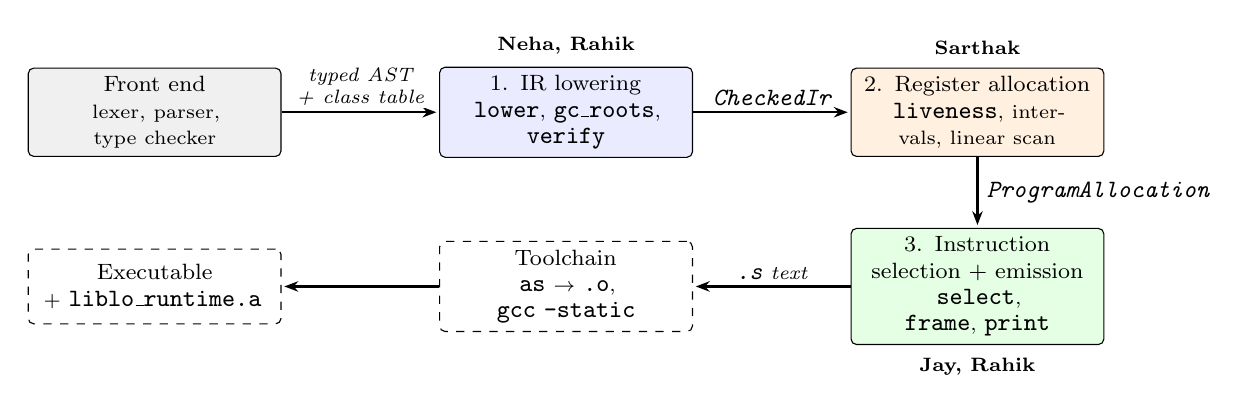
\begin{tikzpicture}[
  font=\footnotesize,
  stage/.style={draw, rounded corners=2pt, align=center, minimum height=0.95cm, text width=3.0cm, inner sep=3pt},
  data/.style={font=\scriptsize\itshape, align=center, fill=white, inner sep=1pt},
  owner/.style={font=\scriptsize\bfseries},
  flow/.style={-{Stealth[length=5pt]}, thick, shorten >=1pt}
]
\node[stage, fill=black!6] (fe) {Front end\\ \scriptsize lexer, parser, type checker};
\node[stage, fill=blue!8, right=2.0cm of fe] (ir) {1. IR lowering\\ \scriptsize \code{lower}, \code{gc\_roots}, \code{verify}};
\node[stage, fill=orange!12, right=2.0cm of ir] (ra) {2. Register allocation\\ \scriptsize \code{liveness}, intervals, linear scan};
\node[stage, fill=green!10, below=0.9cm of ra] (cg) {3. Instruction selection + emission\\ \scriptsize \code{select}, \code{frame}, \code{print}};
\node[stage, dashed, left=2.0cm of cg] (tool) {Toolchain\\ \scriptsize \code{as} $\rightarrow$ \code{.o}, \code{gcc -static}};
\node[stage, dashed, left=2.0cm of tool] (exe) {Executable\\ \scriptsize + \code{liblo\_runtime.a}};

\draw[flow] (fe) -- node[data, above=1pt]{typed AST\\ + class table} (ir);
\draw[flow] (ir) -- node[data, above=1pt]{\code{CheckedIr}} (ra);
\draw[flow] (ra) -- node[data, right=2pt]{\code{ProgramAllocation}} (cg);
\draw[flow] (cg) -- node[data, above=1pt]{\code{.s} text} (tool);
\draw[flow] (tool) -- (exe);

\node[owner, above=1pt of ir] {Neha, Rahik};
\node[owner, above=1pt of ra] {Sarthak};
\node[owner, below=1pt of cg] {Jay, Rahik};
\end{tikzpicture}
\end{center}
Names, field offsets, and vtable layouts live in shared modules (\code{layout.rs}, \code{symbols.rs}, \code{ir/runtime.rs}, \code{ir/statics.rs}), so lowering and codegen share the same definitions. The allocator hands codegen only a map (virtual register $\mapsto$ register or spill slot), a spill count, and the callee-saved registers used. A trivial \code{--spill-all} allocator produces the same map type, which gave us a correct baseline to diff against.

\section{IR and Lowering}
\textbf{Why an IR.} P1's WebAssembly emitter produced assembly directly from the typed AST, without a separate representation for whole-function analysis. WASM hid that cost behind its operand stack and locals. Native code needs a register assignment, which is a whole-function decision made after the whole function exists. The IR is the object that decision is made on.

\textbf{Model.} A \code{FunctionIr} is a list of basic blocks with a single entry. Each block is straight-line instructions followed by exactly one terminator (\code{br}, \code{cbr}, \code{ret}, \code{abort}). Values are mutable virtual registers (not SSA), each typed \code{Int32}, \code{Bool}, \code{Ref} (collectible heap pointer or static ref), \code{Ptr}, or \code{CodePtr(sig)}. Keeping \code{Ref} distinct from \code{Ptr} lets the GC pass find roots without re-deriving types. Instructions are explicit three-address forms: \code{Copy}, \code{Binary}, \code{Unary}, \code{Load [base+off]}, \code{Store}, \code{Call} (direct or indirect), \code{RootStore}, \code{RootLoad}. Operands are virtual registers, immediates, or symbols. A \code{ProgramIr} also carries symbols, interned signatures, and data definitions for \code{.rodata}/\code{.data}.

\textbf{Lowering} is syntax-directed: \code{Builder::expression} returns the \code{Operand} holding the expression's value and appends instructions as a side effect, while \code{statements} builds blocks and wires terminators. Runtime obligations are emitted as explicit IR so later passes see the calls and control flow.

\begin{center}\small
\begin{tabularx}{\linewidth}{@{}l X@{}}
\toprule
\textbf{Source construct} & \textbf{Lowered form} \\
\midrule
\code{new C(args)} & \code{call lo\_alloc(@class\_C)}; store \code{LO\_EMPTY\_STRING} into each String field (inherited ones included); call the constructor \\
\code{r.m(args)} & Evaluate receiver and arguments left to right, then \code{r == null} branches to a block ending in \code{abort lo\_abort\_null\_receiver}; otherwise load descriptor \code{[r+0]}, vtable \code{[desc+48]}, slot \code{[vtable+8k]}, then \code{call\_indirect}. No guard for \code{this.m()} or \code{super.m()}, since \code{this} is never null; every other receiver, including \code{in}/\code{out}/\code{err}, keeps it; \code{super} and I/O calls select their implementations directly \\
reference field assignment & \code{call lo\_gc\_write\_barrier(o, off, v)} performs both the store and barrier \\
\code{a / b}, \code{a \% b} & LO division is total: $x/0=-1$, $x\%0=x$, $x/{-1}=-x$ (wrapping), $x\%{-1}=0$. Divisors $0$ and $-1$ are branched around \code{idiv} in IR (resolved statically for constant divisors), so it can trap neither on $0$ nor on $\mathrm{INT\_MIN}/{-1}$ \\
constructors & explicit constructors run checked \code{this}/\code{super} delegation, then the body; implicit constructors copy their arguments into fields \\
\bottomrule
\end{tabularx}
\end{center}

\code{ProgramIr::verify} returns an immutable \code{CheckedIr} after checking types, control-flow targets, signatures, symbols, definite assignment, root-slot types/bounds, and rejection of raw reference stores except into \code{lo\_bindings}. Guard placement and complete GC-root coverage remain responsibilities of lowering and the root pass.

\textbf{Illustrative dump} (\code{b = new Box(); b.set(7);}, with later uses of \code{b} omitted). The root traffic is explained in \S\ref{sec:frames}.
\begin{lstlisting}
func @lo_method_4_Main_4_main(this:Ref) -> Int32 entry .L0 roots 3 {
.L0:
  t2:Ref = call @lo_alloc(@lo_class_3_Box)
  root_store root0, t2
  call @lo_ctor_3_Box_0(t2)
  t2:Ref = root_load root0           ; reload: a moving GC may have relocated it
  b:Ref = t2
  t3:Bool = b == null
  cbr t3, .L1, .L2
.L1:
  abort @lo_abort_null_receiver(@lo_bytes_0, 3)    ; bytes "set"
.L2:
  t4:Ptr = load [b + 0]              ; class descriptor
  t5:Ptr = load [t4 + 48]            ; vtable
  t6:CodePtr(Ref, Int32) -> Void = load [t5 + 8]    ; slot 1 = set
  root_store root1, b
  call_indirect t6(b, 7)
  b:Ref = root_load root1
\end{lstlisting}

\section{Instruction Selection}
\textbf{Strategy.} Selection is a single forward pass (\code{select\_function}) with one fixed pattern per IR instruction kind. It is not BURS or dynamic-programming tiling: with a $\sim$40-instruction target subset and an IR whose instructions are already one machine-sized operation, a minimal-cost tiler would find almost nothing to merge. The payoff is auditability. Every emitted \code{Inst} is checked against the permitted subset by \code{Inst::check}, including the hand-built \code{main} wrapper.

\textbf{Reserved scratch registers.} \code{rax, rdx, r10, r11} are never allocated (along with \code{rsp, rbp}). \code{rax} is the accumulator and return register, \code{rdx} is overwritten by \code{cdq}/\code{idiv}, and \code{r10}/\code{r11} are scratch for spilled operands, call targets, and parallel-move cycles. This makes every fixup local: no pattern needs a temporary from the allocator or has to evict a live value.

\textbf{Two-address repair.} For $t_2 = t_0 \oplus t_1$ the selector computes in \code{rax}: \code{mov eax, t0; add eax, t1; mov t2, eax}. A spilled right operand can remain in memory when the instruction permits it; scratch registers repair other cases. Comparisons use \code{cmp; setcc al; movzx eax, al}, with signed conditions for integer ordering.

\textbf{Division.} \code{idiv} pins \code{edx:eax}. The selector emits \code{mov r10d, divisor; cdq; idiv r10d}, so the divisor cannot alias \code{eax} or \code{edx}, then reads the quotient from \code{eax} or the remainder from \code{edx}. Both are reserved, so nothing live is clobbered.

\textbf{Widths.} \code{Int32} and \code{Bool} use 32-bit operations; \code{Ref}, \code{Ptr}, and \code{CodePtr} use 64-bit. Widths come from IR operand/result types and the explicit store type. Booleans are zero-extended with \code{movzx eax, al}, and a call's \code{bool} result is re-normalized the same way because System~V leaves the upper bits undefined. \emph{Deviation from the brief:} there is no \code{movsxd}. Pointers are always 64-bit values and field offsets are compile-time immediates, so no runtime 32$\to$64 sign extension arises. \code{lea} forms RIP-relative symbol addresses and stack-frame addresses, not LO integer arithmetic.

\textbf{Addressing and dispatch.} Loads and stores use \code{[base + disp]} with displacements from \code{layout.rs}. Virtual dispatch loads the object's descriptor, the descriptor's vtable, and the slot's code pointer followed by \code{mov r11, fn; call r11}. Static data is addressed RIP-relative. The numeric offsets shown above come from the shared native layout: ABI-aligned headers and descriptors, with pointer-sized field and vtable slots.

\section{Liveness and Linear-Scan Allocation}
\textbf{Dataflow.} Liveness is a backward analysis iterated to a fixed point over the blocks in reverse order:
\[
  \mathrm{OUT}[B] = \bigcup_{S \in \mathrm{succ}(B)} \mathrm{IN}[S],
  \qquad
  \mathrm{IN}[B] = \mathrm{USE}[B] \cup \bigl(\mathrm{OUT}[B] \setminus \mathrm{DEF}[B]\bigr),
\]
where $\mathrm{USE}[B]$ holds registers read before any definition in $B$. Registers are not SSA, so DEF acts as a kill per block.

\textbf{Intervals.} Blocks are linearized in layout order and every instruction and terminator receives a position. Each virtual register becomes \emph{one} conservative interval $[\text{start},\text{end}]$ (inclusive) from its first definition or live-in to its last use or live-out. This is safe across branches and loops, at the cost of filling in holes.

\textbf{Dead copies.} Before GC-root insertion and register allocation, a backward liveness pass removes \code{Copy} instructions whose destinations are not live afterward. This removes unused default initializations and overwritten copies before they can extend intervals and cause unnecessary spills. Calls and other potentially effectful instructions are preserved; the spill policy is unchanged.

\textbf{Allocation} follows Poletto and Sarkar. Intervals are processed by increasing start. \code{expire\_finished\_intervals} frees registers whose interval ended. If a usable register is free, the interval takes the first one in pool order. Otherwise \code{spill\_at\_interval} compares against the active interval with the \emph{furthest end} among those holding a usable register: if that one ends later it is evicted and its register reused, and otherwise the new interval is spilled. A spilled register lives in its stack slot for its whole lifetime.

\textbf{Registers and calling convention.} The pool has ten registers, ordered \code{rsi, rdi, r8, r9, rcx} (caller-saved) then \code{rbx, r12--r15} (callee-saved). Reserved are \code{rsp, rbp} and the four scratch registers above. The calling-convention rule is applied \emph{per value}: a value that is read after some call returns (\code{live\_across\_calls}) may use only callee-saved registers or a spill slot, while every other value may use any register, caller-saved first because those need no save or restore. In a function that makes calls, parameters also count as surviving a call, because \code{lo\_push\_frame} runs in the prologue after the parameter moves. A callee-saved register is saved to a frame slot and restored only if it ends up in the final map. Because \code{gc\_roots} reloads every \code{Ref} from its root slot after each call, a \code{Ref}'s pre-call register is never read again, so those reloads end pre-call reference lifetimes; parameters still obey the prologue constraint, including \code{Ref} parameters. This replaces call-site splitting and save/restore code.

Some argument registers are allocatable, so values can sit in \code{rdi}, \code{rsi}, \code{rcx}, \code{r8}, \code{r9}. Call setup therefore writes the register arguments with the same \code{moves.rs::parallel\_move} used for incoming parameters, which orders the moves and breaks cycles through \code{r10}. An indirect call target is loaded into \code{r11} first, before any argument register is overwritten. Fixed-register constraints from \code{idiv} and \code{rax} results are served by the reserved set.

\textbf{Linear scan versus graph coloring.} Chaitin--Briggs builds an interference graph (up to $O(N^2)$ edges), then loops through simplify, potential-spill, select, and conservative coalescing, rebuilding the graph after each actual spill. It can reduce spills and copies through coalescing and more precise interference. For a fixed register pool, our interval allocation is $O(N\log N)$ including sorting, separate from fixed-point liveness, but the deciding factor was ease of implementation: we want to be able to read and understand all of the code we wrote, and linear scan is a single pass over sorted intervals that is much simpler than building, simplifying, and coalescing a graph. We checked correctness against \code{--spill-all}. This is a design argument; we did not implement or benchmark a graph-coloring allocator.

\section{Stack Frames, GC Protocol, and Emission}\label{sec:frames}
\textbf{Frame layout.} \code{Frame} owns stack offsets; shared \code{layout.rs} definitions own object and descriptor offsets.
\begin{lstlisting}
[rbp + 16 + 8k]  stack argument k (7th onward)
[rbp + 8]        return address
[rbp]            saved rbp
[rbp - 8(i+1)]   saved callee-saved register i
                 ShadowFrame { parent, num_roots, roots[] }  (only if function calls)
                 spill slots, 8 bytes each
                 ret_save                                    (only if function calls)
                 padding: rsp = 0 (mod 16) at every call
\end{lstlisting}
Stack-passed arguments are pushed right to left with one pad slot when the count is odd, and cleaned up after the call.

\textbf{GC safepoints.} Every call may allocate, and a moving collector relocates objects, so a \code{Ref} held in a register may be stale after a call. The protocol is split between IR and codegen:
\begin{enumerate}
  \item \code{ir/gc\_roots.rs} finds the \code{Ref}s live across each call (using the same liveness analysis) and inserts \code{root\_store slot, v} before the call and \code{root\_load} into the register after it. It also nulls the pass's other slots so stale pointers are never scanned.
  \item The prologue builds the \code{ShadowFrame} in the native frame, zeroes \code{roots[]}, and calls \code{lo\_push\_frame}. The epilogue saves the return value, calls \code{lo\_pop\_frame}, and restores it. Functions with no calls skip all of this.
\end{enumerate}
Because roots are ordinary IR instructions, the allocator needs no GC knowledge and \code{verify} can check slot bounds and types.

\textbf{Emission and toolchain.} \code{emit\_program} produces \code{.text} (one function per \code{FunctionIr}, labels namespaced by function). \code{emit\_data} produces \code{.rodata} (class descriptors, vtables, names, string literals) and \code{.data} (\code{lo\_bindings}, the static root frame for \code{in}/\code{out}/\code{err}). Only \code{print.rs} formats assembly text, and that text is the compiler's final output. A synthesized \code{main} (\code{push rbp; mov rbp, rsp; call lo\_runtime\_init; call lo\_entry; pop rbp; ret}) initializes the runtime and then calls the lowered IR function \code{lo\_entry}. \code{lo\_entry} uses ordinary lowered IR and the normal frame machinery: it pushes the \code{lo\_bindings} frame, allocates \code{in}/\code{out}/\code{err}, constructs \code{Main}, calls \code{Main.main} directly (\code{Main} cannot be extended and \code{lo\_alloc} never returns null, so no dispatch or null check is needed), pops the frame, and returns the exit code in \code{eax}. \code{gcc -static} supplies the C startup code, which uses \code{main}'s return value as the process exit status. We do not implement a linker. \code{assemble\_and\_link} writes the \code{.s} file, runs \code{as} to produce a \code{.o}, and lets \code{gcc -static} link it against \code{liblo\_runtime.a}, so runtime symbols resolve at link time. The grading contract instead emits assembly for the grader to link against its runtime.

\section{Verification and Limitations}
Both allocators are CLI-selectable (\code{--linear-scan} default, \code{--spill-all} baseline), so any program can be built both ways and checked against \code{tests/expected/}. \textbf{Limitations:} whole-interval spills; no splitting, coalescing, or peephole pass.

\end{document}
